\documentclass[12pt]{article}

\usepackage[dvips,letterpaper,margin=0.75in,bottom=0.5in]{geometry}
\usepackage{cite}
\usepackage{slashed}
\usepackage{graphicx}
\usepackage{amsmath}
\usepackage{braket}

\usepackage[american,fulldiode]{circuitikz}
\usetikzlibrary{calc}

\newcommand{\kb}{k_{\rm b}}
\begin{document}
\ctikzset{bipoles/thickness=1}
\ctikzset{bipoles/resistor/height=.115}
\ctikzset{bipoles/resistor/width=.3}
\ctikzset{bipoles/capacitor/height=.2}
\ctikzset{bipoles/capacitor/width=.06}

\title{Muon Decay}
\author{Michael Mulhearn}

\maketitle

\section{Introduction}

\begin{figure}[htbp]
\begin{center}
{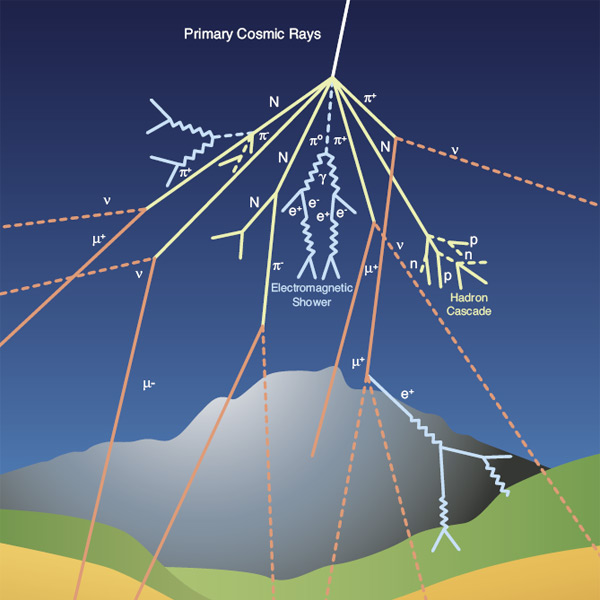
\includegraphics[width=0.35\textwidth]{figs/cosmic_ray.jpg}}\\
\end{center}
\caption{\label{fig:cosmic}  Cosmic ray shower induced by a primary cosmic ray (typically protons) striking an atom in the upper atmosphere.}\end{figure}

The muon is a fundamental particle in the Standard Model of particle physics.  It is essentially a heavier version of the electron.  Like the electron, the muon has a corresponding anti-particle, the anti-muon ($\mu^+$).  Muons are readily available for study because they are produced as a result of showers that are induced by incident cosmic rays that constantly bombard the earth.  Typical primary cosmic rays are protons, and there collisions with nuclei in the upper atmosphere produce mainly protons, neutrons, and pions.  The subsequent decays of these particles produce electrons, neutrinos, and the muons we will be studying.  The flux of muons at sea-level is about 1 per ${\rm cm}^2$ per minute, and this population has a mean kinetic energy of about $4~\rm GeV$.  Such muons are highly penetrating:  they pass quite readily through buildings.

The muon decays via the weak interaction, its most probable decays being:
\begin{eqnarray*}
\mu^- \to e^- + \bar{\nu}_e \nu_\mu,\\
\mu^+ \to e^+ + \bar{\nu}_\mu \nu_e.
\end{eqnarray*}
As fundamental particles, muons are indistinguishable from one another, and therefore the decay rate for a population of $N$ muons must be simply proportional to $N$:
\begin{displaymath}
\frac{dN}{dt} = -\frac{N}{\tau}
\end{displaymath}
The solution to this differential equation is:
\begin{displaymath}
N(t) = N(0) \exp(-t/\tau).
\end{displaymath}
In this lab, you will measure the lifetime of the muon, which has the value 
\begin{displaymath}
\tau_\mu = 2.1969811(22) \mu s
\end{displaymath}
in vacuum as reported by the Particle Data Group (PDG) with the uncertainty in parenthesis.   Interactions with the scintillator material in this experiment lead to a slightly different expectation for the lifetime as discussed below.

Muons are produced at a typical height $15~\rm km$ above sea-level, and so, in the earth frame, their transit time from the upper atmosphere to our lab is therefore about $50~\rm \mu s$ or about 20 lifetimes.
The fact that we see an appreciable number of them at sea level, given an upper limit on their production rate in the atmosphere, is clear evidence for time dilation.

\section{Experimental Setup}

\begin{figure}[htbp]
\begin{center}
{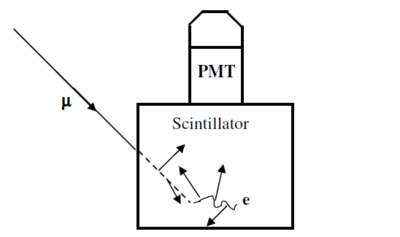
\includegraphics[width=0.55\textwidth]{figs/setup.png}}\\
\end{center}
\caption{\label{fig:setup}  Experimental setup.}\end{figure}

The active component of the particle detector used in this experiment is a polyvinyltoluene-based plastic scintillator in the shape of a cylinder with a $15~\rm cm$ diameter and a $12.5~\rm cm$ height.  All materials absorb energy due to the passage of ionizing radiation.  Scintillators are materials which re-emit a fraction of this energy as visible light, typically in the blue to near UV range.   The light yield is relatively low, so a sensitive photomultiplier tube is used to amplify a modest number of photons into a large easily measurable voltage. 

Muons are therefore constantly passing through the scintillator, depositing energy, and causing observable PMT pulses which are recorded by the data acquisition system (DAQ\footnote{Which for this one time, you don't have to build yourself!}).  Occasionally, however, a relatively low-energy muon enters the scintillator and deposits {\em all of it's kinetic energy}, coming to rest.  As an unstable particle, it eventually decays into a highly-energetic electron and neutrinos.  The electron deposits additional energy in the scintillator which is observed as a second pulse.  The DAQ records the digitized time interval between these two pulses, which you will analyze to determine the muon life time.

\section{Muon Lifetime Analysis}

\begin{figure}[htbp]
\begin{center}
{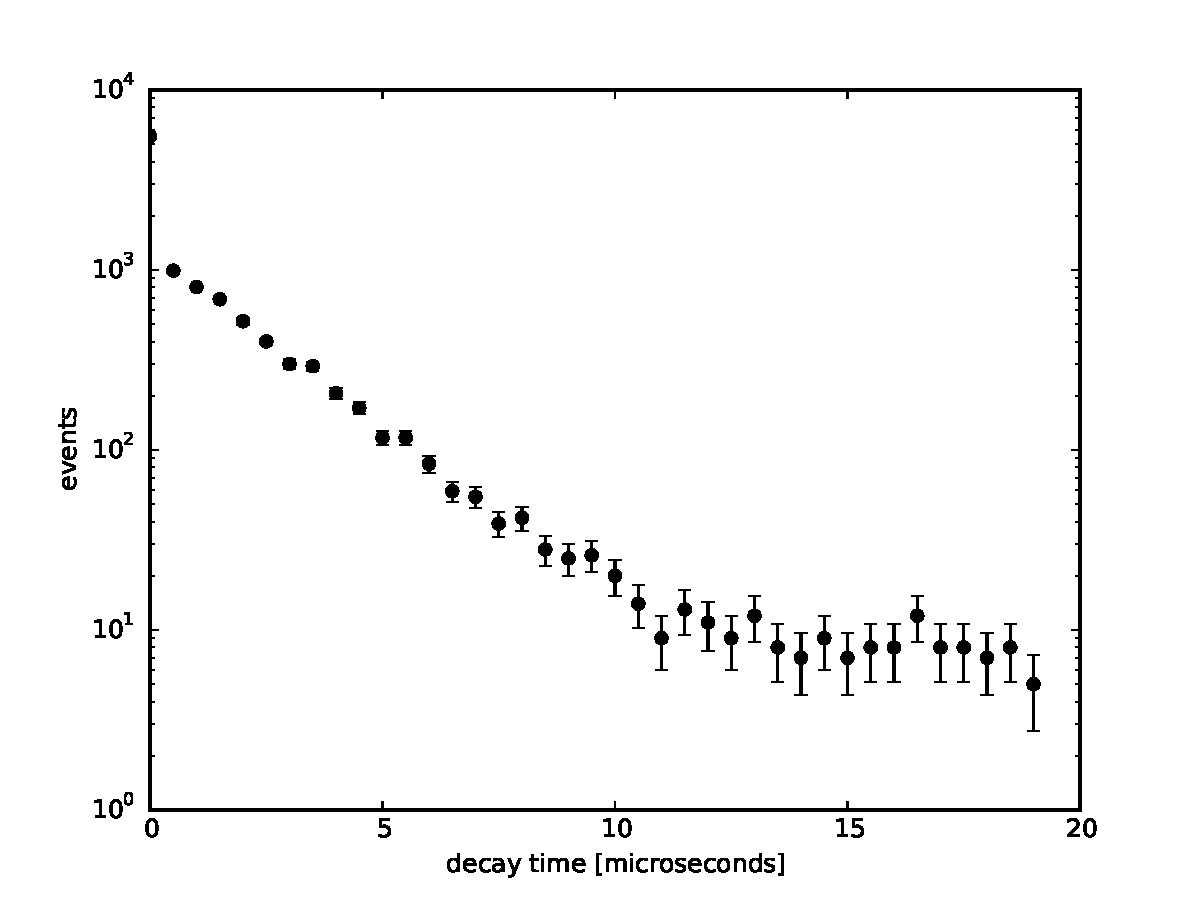
\includegraphics[width=0.65\textwidth]{figs/muon.pdf}}\\
\end{center}
\caption{\label{fig:muon}  The muon decay data collected for this experiment.}\end{figure}

We don't have experimental control over the number of muons that enter the scintillator, let alone the number that come to rest.   Instead, our data consists of $N$ recorded events.  In the vast majority of these events, the value recorded from the TDC (time to digital converter) for the time between two pulses will be saturated (at the maximum value) indicating that a second pulse was not detected during the observable time window.  But a subset of these events will consist of a non-saturated time interval, indicating that two distinct pulses were observed separated by the recorded time interval.  This time interval, the decay time of the muons in this population, will have a time-dependence given by:
\begin{displaymath}
-\frac{dN}{dt} = \frac{N(0)}{\tau} \exp(-t/\tau)
\end{displaymath}
which you will use to extract the muon life time.  This is possible because the muon decay rate ($\lambda$)
and it's lifetime $\tau$ are simply recipocrals:
\begin{displaymath}
\lambda \equiv \frac{-\frac{dN}{dT}}{N(t)} = \frac{1}{\tau}.
\end{displaymath}

There is a source of background for these two hit events, which arises from the possibility for two muons to arrive independently within the time window for observation $T$.  You will determine this background due to the fact that it is flat in time.

%We can make two predictions about this background:
%\begin{itemize}
%\item Any event has a probability to contain such a second hit which is simply $rT$ where $r$ is the rate of single muons entering the scintillator and $T$ is the timing window.
%\item It should be flat as a function of time.
%\end{itemize}

The data already collected for you for this experiment is shown in Fig.~\ref{fig:muon}.  You can reproduce this plot using the python script provided on the course website along with the raw data file.  On this semi-log plot you can clearly see the flat background (zero slope region) and the exponential decay (negative slope region).  You can also see an additional instrumental background producing an excess of entries in the first bin.  You should avoid this background by removing the first bin from your fit.  By fitting this curve appropriately, you should determine the muon lifetime.

%\section{Muon / Anti-Muon Ratio}

%Due to additional decay processes when captured by an atomic nucleus, the decay time of the negatively %charged muon in matter is lower than its free space value:
%\begin{eqnarray*}
%\tau_- &=& 2.043(3) \times 10^{-6} \mu s \\
%\tau_+ &=& 2.1969811(22) \times 10^{-6} \mu s
%\end{eqnarray*}
%where we have used the measured values in carbon, which should be close to value for our organic %scintillator.

%As discussed in class, you can determine the ratio $\rho$ of anti-muons to muons from the relation:
%\begin{displaymath}
%\rho = - \frac{\tau_+}{\tau_-} \cdot \frac{\tau_- - \tau}{\tau_+ - \tau}
%\end{displaymath}
%where $\tau$ is the measured valued of the muon lifetime.

\section{Lab Write-up}

For this lab write-up, you only need to describe your analysis. 

You should fit the muon lifetime distribution, report the fitted values, and plot the resulting distribution along with the data.  An example script using Scientific python to fit simulated data to a straight line is available on the course website.

You should report the statistical uncertainty on the fitted value for the muon lifetime.    In addition, there are several systematic uncertainties associated with the experiment.  The largest is the effect of material interactions on the lifetime of the muon, which is about $5\%$.   Other systematic effects are smaller, and can be neglected.

Due to the limited time available to complete this analysis, there is no requirement to provide Monte Carlo studies, although you are certainly welcome to provide them.

\end{document}


